% Fig. 1, the two models (TikZ, standalone)
% Compile: pdflatex fig1_architecture.tex  ->  fig1_architecture.pdf
% Width under the 12.2 cm LNCS \textwidth, so it is included at 100 per cent
% and the smallest text stays 7 pt (\scriptsize), above Springer's 6 pt minimum.
\documentclass[border=2pt]{standalone}
\usepackage[T1]{fontenc}
\IfFileExists{lmodern.sty}{\usepackage{lmodern}}{}
\usepackage{tikz}
\usetikzlibrary{arrows.meta, positioning, calc}

% the same two colours as the matplotlib figures
\definecolor{cpool}{HTML}{262626}
\definecolor{cattn}{HTML}{C8372D}

\begin{document}
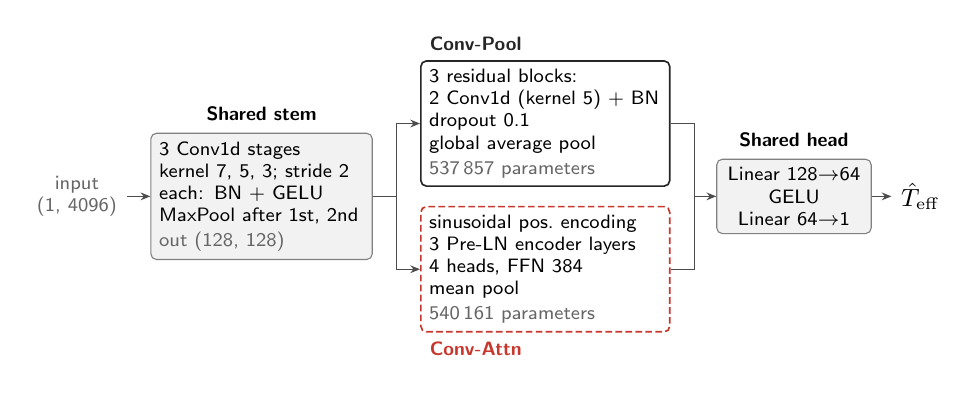
\begin{tikzpicture}[
    font=\sffamily\scriptsize,
    >={Stealth[length=3.5pt, width=2.8pt]},
    node distance=0.42cm,
    every node/.style={align=center},
    arr/.style={->, draw=black!70, line width=0.5pt},
    blk/.style={draw=black!50, fill=black!5, rounded corners=2pt,
                inner xsep=3pt, inner ysep=3pt, align=left},
    title/.style={font=\sffamily\scriptsize\bfseries},
    tensor/.style={font=\sffamily\scriptsize, text=black!60},
  ]

% ---- shared stem -------------------------------------------------------------
\node[blk, text width=2.6cm] (stem) {%
  3 Conv1d stages\\
  kernel 7, 5, 3; stride 2\\
  each: BN + GELU\\
  MaxPool after 1st, 2nd\\[1pt]
  {\color{black!60}out (128, 128)}};
\node[title, above=1pt of stem] {Shared stem};

\node[tensor, left=0.30cm of stem] (in) {input\\(1, 4096)};
\draw[arr] (in) -- (stem);

% ---- the two bodies ----------------------------------------------------------
\coordinate (split) at ($(stem.east)+(0.30,0)$);

\node[blk, draw=cpool, line width=0.6pt, fill=white, text width=2.95cm,
      anchor=south west] (pool) at ($(split)+(0.30,0.12)$) {%
  3 residual blocks:\\
  2 Conv1d (kernel 5) + BN\\
  dropout 0.1\\
  global average pool\\[1pt]
  {\color{black!60}537\,857 parameters}};
\node[title, anchor=south west, text=cpool] at (pool.north west) {Conv-Pool};

\node[blk, draw=cattn, line width=0.6pt, dash pattern=on 2.4pt off 1.2pt,
      fill=white, text width=2.95cm, anchor=north west] (attn)
      at ($(split)+(0.30,-0.12)$) {%
  sinusoidal pos.\ encoding\\
  3 Pre-LN encoder layers\\
  4 heads, FFN 384\\
  mean pool\\[1pt]
  {\color{black!60}540\,161 parameters}};
\node[title, anchor=north west, text=cattn] at (attn.south west) {Conv-Attn};

\draw[line width=0.5pt, draw=black!70] (stem.east) -- (split);
\draw[arr] (split) |- (pool.west);
\draw[arr] (split) |- (attn.west);

% ---- shared head -------------------------------------------------------------
\coordinate (merge) at ($(pool.east |- stem.east)+(0.30,0)$);
\draw[line width=0.5pt, draw=black!70] (pool.east) -| (merge);
\draw[line width=0.5pt, draw=black!70] (attn.east) -| (merge);

\node[blk, text width=1.75cm, right=0.28cm of merge, align=center] (head) {%
  Linear 128$\to$64\\GELU\\Linear 64$\to$1};
\node[title, above=1pt of head] {Shared head};
\draw[arr] (merge) -- (head);

\node[right=0.25cm of head, font=\small] (out) {$\hat{T}_{\mathrm{eff}}$};
\draw[arr] (head) -- (out);

\end{tikzpicture}
\end{document}
